We assess our interpretability scores against a variety of alternative methods for finding dictionaries of features in language models. In particular, we compare interpretability scores on our dictionary features to those produced by a) the default basis, b) random directions, c) Principal Component Analysis (PCA), and d) Independent Component Analysis (ICA). For the random directions and for the default basis in the residual stream, we replace negative activations with zeros so that all feature activations are nonnegative \footnote{
For PCA we use an online estimation approach and run the decomposition on the same quantity of data we used for training the autoencoders. For ICA, due to the slower convergence times, we run on only 2GB of data, approximately 4 million activations for the residual stream and 1m activations for the MLPs.}.

% Sparse coding differs significantly to the aforementioned baselines in that it has a bias and then a ReLU applied to the direction which allows it to be sensitive to smaller regions of the activation space. This removes some of the noise from the activations which could make it easier to predict a high proportion of the variance. To ensure we are comparing to fair baselines, we create Top-K versions of PCA and ICA in which only the top K directions most relevant to a given datapoint are retained, and the rest are set to zero. We select K to match the average number of features active per token for the learned dictionary with ratio 1 and l1 $\alpha$ of 8e-4.

\begin{figure}
    \centering
    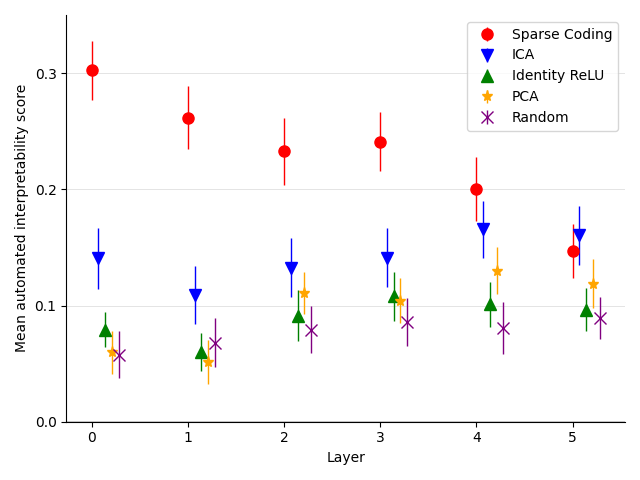
\includegraphics[scale=0.6]{images/residual_top_random_means_and_cis_new.png}
    \caption{Average top-and-random autointerpretability score of  our learned directions in the residual stream, compared to a number of baselines, using 150 features each. Error bars show 95\% confidence intervals around means. The feature dictionaries used here were trained for 10 epochs using $\alpha=.00086$ and $R=2$.}
    \label{fig:main_interp_scores_comparison}
\end{figure}


Figure \ref{fig:main_interp_scores_comparison} shows that our dictionary features are far more interpretable by this measure than dictionary features found by comparable techniques. We find that the strength of this effect declines as we move through the model, being comparable to ICA in layer 4 and showing minimal improvement in the final layer.

This could indicate that sparse autoencoders work less well in later layers but also may be connected to the difficulties of automatic interpretation, both because by building on earlier layers, later features may be more complex, and because they are often best explained by their effect on the output. \citet{bills2023language} showed that GPT-4 is able to generate explanations that are very close to the average quality of the human-generated explanations given similar data. However, they also showed that current LLMs are limited in the kinds of patterns that they can find, sometimes struggling to find patterns that center around next or previous tokens rather than the current token, and in the current protocol are unable to verify outputs by looking at changes in output or other data. 

We do show, in Section \ref{section:case_studies}, a method to see a feature's causal effect on the output logits by hand, but we currently do not send this information to the language model for hypothesis generation. The case studies section also demonstrates a closing parenthesis dictionary feature, showing that these final layer features can give insight into the model's workings.

See Appendix \ref{appendix:full_autointerp} for a fuller exploration of different learned dictionaries through the lens of automatic interpretability, looking at both the MLPs and the residual stream.